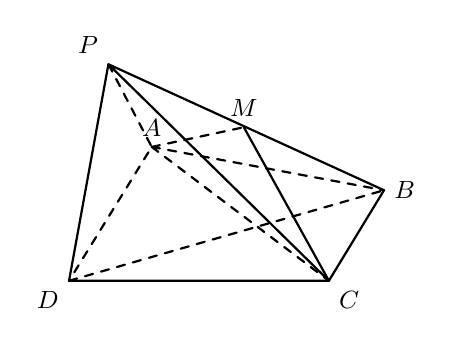
\begin{tikzpicture}[thick,line cap=round,line join=round,
  every node/.style={font=\small}]
  \coordinate (P) at (0,2.75);
  \coordinate (D) at (-.5,0);
  \coordinate (C) at (2.8,0);
  \coordinate (B) at (3.5,1.15);
  \coordinate (A) at (.55,1.7);
  \coordinate (M) at (1.72,1.95);
  \draw (P)--(D)--(C)--(B)--(P)--(C);
  \draw (M)--(C);
  \draw[dashed] (P)--(A)--(D) (A)--(B) (A)--(C) (A)--(M) (D)--(B);
  \node[above left] at (P) {$P$};
  \node[above] at (A) {$A$};
  \node[right] at (B) {$B$};
  \node[below right] at (C) {$C$};
  \node[below left] at (D) {$D$};
  \node[above] at (M) {$M$};
\end{tikzpicture}
